V předchozí kapitole jsme se seznámili s technickými principy a postupy, které se uplatňujív BigData konceptu. V tét kapitole se budu zabývat jedním z hlavních témat práce a tou je open source řešení pro platformu BigData od organizace Apache Foundations, také známý jako Apache Big Data stack. Tento stack se skládá z několika aplikací, které až na jednu výjimku na sobě nejsou nikterak závislé. V záběru této kapitoly se budu důkladně věnovat pro nás nejdůležitější části tohoto stacku a tím je NoSQL databázový systém Cassandra.

\section{Hadoop}




Hadoop je softwarová knihovna napsaná v programovacím jazyce Java a umožňuje distribuované zpracování velkého množství dat napříč clusterem pomocí jednoduchých programovacíh modelů- Je navržený aby dobře škáloval cluster tvořící jeden až několik tisíc počítačů, kde každý nabízí lokální výpočetní výkon a úložiště dat. Hadoop řeší problémy s hardwarem na aplikační vrstvě a tudíž je možné navrhovat vysoce dostupné služby na clusterů počítačů, aniž bychom se museli strachovat výpadků. Jeho 4 komponenty tvoří nejpodstatnější část pro celou analytickou práci s  daty. A všechny ostatní aplikace přímo, čí nepřímo některé části Hadoopu používají nebo jsou na nich dokonce založeny. Jaké tedy jsou tyto 4 komponenty hadoopu ?


\begin{figure}[h]
\centering

\includegraphics[scale=0.15]{images/hadoop}
\caption{Logo Apache hadoop}
\label{fig:yarn}

\end{figure}


\subsection{Hadoop Commons}
Jedná se pouze o základní sadu nástrojů podporujícíc a propojující ostatní moduly Hadoopu.


\subsection{Hadoop File System (HDFS)}
Jedná se o open source distribuovaný filesystém, jehož některé prvky vychází z dříve zmíněného GFS. HDFS umožňuje uložit velké množství dat mezi jednotlivé uzly.  HDFS umožňuje velice dobré škálování s rostoucím objemem dat. Ostatní technologie z Apache Big Data Stacku filesystém využívají ke sběru a ukládání výsledků jejich analytických procesů. HDFS cluster se skládá primárně z NameNode, který řídí filesystemová metadata a z DataNodů, které data uchovávají. 

\subsection{Hadoop MapReduce}
MapReduce jsme zmínili výše a jen zopakuji, že se jedná o programovací paradigma a framework na paralelní zpracování dat. Nabízí API, díky kterému můžeme jednoduše programovat naše vlastní MapReduce operace. Tento framework nabízí základní kostru, kterou programátor doplní a o vše ostatní se stará samotná knihovna. Přesto všakveškerá logika programu zavisí na programátorovi. 

\subsection{Hadoop YARN}
Tento modul se stará o plánování jednotlivých MapReduce programů a o správu dostupných zdrojů v celém clusteru a rozhoduje jaká data se kam budou posílat a počítat. Základní Architektura YARNu má za myšlenku mít jeden globální uzel, který se nazývá \uv{Resource Manager} a Pro každý běh aplikace mít tzv. \uv{Application Master}, který má na starosti komunikaci s \uv{Node Managery} a dohlížením nad spouštěním jednotlivých Tasků. Resource Manager se skládá ze 2 hlavních komponent Plánovače a Aplikačního manažera. Plánovač je zodpovědný za alokování zdrojů pro různé běžící aplikace. Aplikační manažer je zodpovědný za příjem nových MapReduce programů a jejich správné zařazení. NodeManager je agent běžící na každém stroji, která je zodpovědný za aplikační kontejnery a monitoruje stav dostupných prostředků stroje a ohlašuje se Resource Manageru, který tak má potřebné informace k přerozdělování nových úkolů.

\begin{figure}[h]
\centering
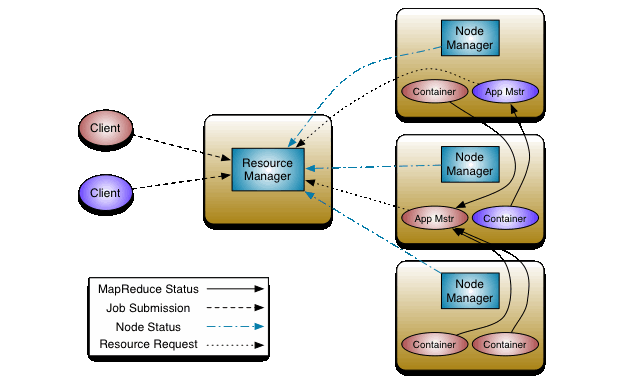
\includegraphics[scale=0.7]{images/yarn_architecture}
\caption{Architektura Hadoop YARN}
\label{fig:yarn}

\end{figure}



\newpage 

\section{HBase}
Je NoSQL databázový systém, který je založený na principu Google BigTable. Jedná se o druhou nejpoužívanšjí NoSQL databázi v Apache Big Data Stacku. Implementačně je zavíslá na HDFS, který používá k ukládání dat. Výhodou je velice jednoduhá a rychlá integrace s Hadoop MapReduce. HBase sdědil po Hadoopu i jeho Master-Slave architekturu.


\section{Hive}


Apache Hive je data warehouse infrastruktura postavená na vrchu Hadoopu na poskytování analýzy a dotazování se nad daty. Původně byl tento software vyvinut ve společnosti Facebook. A nyní se jeho starají společnost jako je NetFlix a Amazon. Hive podporuje anaýzu velkých datasetů uložených v HDFS nebo HDFS-kompatibilních systémech jako například (CassandraFS nebo Amazon S3). Syntaxe jeho dotazovacího jazyka HiveQL je velice podobná SQL a proto ho mohou inženýři ovládající tento jazyk velice brzy ovládnout.HiveQL nabízí programátorům prostředky, které nejsou běžně v NoSQL databázích dostupné jako například funkce JOIN. 

\begin{wrapfigure}{r}{0.5\textwidth}
  \centering
    
\includegraphics[scale=0.5]{images/hive_logo}
\caption{Logo Apache Hive}

\end{wrapfigure}

Hive funguje na principu, že si dotaz přeloží a převede do kodu kompatibilního s Hadoop Mapreduce a výsledný program následně spustí na Hadoop clusteru. Obrovskou výhodou je, že programátor dostává v podstatě s nulovým snažením hotový MapReduce program, který by jinak musel zdlouhavě psát, což umožnuje být vysoce efektivní. Hive si standardně ukládá metadata do embedované databáze Derby. Podporuje pokročilejší funkce jako například Indexy, kompresi nebo uživatelem definované funkce (UDF) samozřejmostí jsou standardní matematické a řetězcové funkce aplikovatelné v HiveQL dotazech. 



\section{Pig}


Pig funguje na stejném principu jako Hive. Tedy , že převede vámi napsaný kód do hotového MapReduce řešení a tento kód spustí nad Hadoop clusterem. Tato knihovna byla napsána ve firme Yahoo a později opensourcována pod Apache foundation. Pig používá svůj vlastní jazyk pojmenovaný Pig Latin a oproti HiveQL nemá s SQL moc společných rysů. Latin se spíše podobá funkcionálním jazykům. Pig a Hive dělají tedy stejné věci, tak proč používat obojí? Je to spíše volba osobních preferencí, či preferencí vašeho vývojářského týmu. S oběma technologiemi lze dosáhnout stejných výsledků. Přesto má Pig lepší uplatnění v případě tvorby komplikověnšjích data flow a HiveQL se více hodí pokud jsou potřeba Ad-Hoc dotazy. Přestože lze dosáhnout stejných výsledků s oběmi platformami, určitě doporučuji umět obě a použít Hive nebo Pig v konkrétních siuacích, kde mají lepší užití. 



\section{SolR}

Solr [Solar] je vyhledávací platformou odvozenou od Apache Lucene. Mezi její hlavní výhody patří:

\begin{itemize}
\item Pokročilý full-text vyhledávací engine
\item Optimalizace pro vysokoobjemový tok dat
\item Otevřené rozhraní pomocí XML,JSON nebo HTTP
\item Lineární škálovatelnost, automatická replikace indexu, auto failover a samoobnovení
\item Indexace v témeř reálném čase
\item Možnost doprogramování vlastních pluginů
\end{itemize}

Solr využívá Lucene index, což znamená, že je formát je striktně definovaný. Změna ve formátu indexu znamená reindexaci celého dokumentu. Díky lehkému nastavení a možnostem výstupu a pokročilými funkcemi jako je například GeoSpatial vyhledávání nebo facetové full text hledání, je SolR v komerční a open source sféře vyhledávacím enginem číslo 1.


\section{Squoop}

Tento nástroj je velice užitečný, protože ne vždy chceme mít všechna data pouze v NoSQL databázích a pokud to je možné, využití výhod relačních databází je logickou volbou. Apache Squoop je nástroj pro hromadnou migraci z HDFS (či kompatibilního) file systému do strukturovaných úložišt jako například: relačních databází. Přesun dat je navržený obousměrně stejně tak můžeme využít Squoop k migraci dat z  relačních databází do HDFS (a kompatibilních) systémů. Výhodou je vysoká efektivita a nízká časová investice oproti psaní vlastních migračních scriptů.

\section{Mahout}

Mahout je slovo, které pochazí z Hindi a jeho překladem do češtiný získáme spojení jezdec na slonovi. Slonem se v BigData komunitě myslí projekt Apache Hadoop, který má slona ve svém logu a je s tímto zvířetem neodmyslitelně spojený. Projekt Mahout se snaží svým metaforickým názvem naznačit využívání hadoopu k vytvoření knihovny pro podporu škálovatelného \uv{Machine learningu}. Mahout je sada funkcí a algoritmů využívaných v odvětví machine learningu, naprogramovaných pomocí Hadoop MapReduce paradigmatu. Primární zaměření Mahoutu je na odvětví kolaborativního filterování, clusterování a klasifikace dat. Mahout také obsahuje vysoké množství matematických funkcí a algoritmů z oblasti lineární  algebry a statistiky. V současné době lze využít Mahout na tyto základní způsoby užití. Doporučovací funkce na základě uživatelského chování, rozřazování dokumentů do clusterů na základě shody v obsahu a Klasifikace dokumentů na základě již uložených kategorizovaných dokumentů. 

\section {ZooKeeper}

Autoři projektů v rámci Apache foundations a především ti zaměření na projekty BigData stacku mají pro metafory a různá symbolická spojení velkou slabost. Jak názvy a loga projektů napovídají, velká část projektů má v názvu nebo logu nějaké zvíře, či referenci na něj. Zároveň uhlídat a spravovat byť malý ale distribuovaný systém, může být velký chaos a proto je potřeba ten správný hlídač. ZooKeeper v překladu tedy hlídač zoo je nástroj pro správu a konfiguraci distribuovaných systému z platformy Apache BigData. 

